\documentclass[t]{beamer}
\usetheme[english]{KIT}

\usepackage{amssymb} %% For \backprime
\usepackage{multicol}

%\usepackage{mathpartir}
\usepackage{graphicx}

\usepackage{tikz}
\usetikzlibrary{arrows.meta,positioning,calc}

\usepackage[T1]{fontenc}
\usepackage{babel}
\usepackage{booktabs}
\usepackage[normalem]{ulem}
\usepackage{fontspec}
\setmonofont[Scale=MatchLowercase]{Iosevka}
%\newfontfamily\lc[Scale=MatchLowercase]{Iosevka SS09}

\usepackage{minted}
\definecolor{codebg}{rgb}{0.95,0.95,0.95}
\setminted{bgcolor=codebg,breaklines}
\usemintedstyle{tango}
\newmintinline[lean]{lean}{bgcolor=white}
\newminted{lean}{fontsize=\footnotesize}

\usepackage{newunicodechar}
\newfontfamily{\freeserif}{DejaVu Sans}
\newunicodechar{ℕ}{\freeserif{ℕ}}
\newunicodechar{ℝ}{\freeserif{ℝ}}
\newunicodechar{ₐ}{\freeserif{ₐ}}
%\newunicodechar{₁}{\freeserif{₁}}
%\newunicodechar{∈}{\freeserif{∈}}
\newunicodechar{𝓞}{\ensuremath{\mathcal{O}}}
\newunicodechar{∉}{\freeserif{∉}}
%\newunicodechar{Π}{\freeserif{Π}}
%\newunicodechar{→}{\freeserif{→}}
\newunicodechar{⦃}{\freeserif{⦃}}
\newunicodechar{⦄}{\freeserif{⦄}}
%\newunicodechar{∧}{\freeserif{∧}}
%\newunicodechar{∨}{\freeserif{∨}}
%\newunicodechar{⊢}{\freeserif{⊢}}
\newunicodechar{⊑}{\freeserif{⊑}}
\newunicodechar{ₚ}{\freeserif{ₚ}}
\newunicodechar{∘}{\freeserif{∘}}
\newunicodechar{ₗ}{\freeserif{ₗ}}
\newunicodechar{∪}{\freeserif{∪}}
\newunicodechar{⋃}{\freeserif{⋃}}
\newunicodechar{𝓸}{\ensuremath{o}}
\newunicodechar{⊆}{\freeserif{⊆}}
\newunicodechar{≼}{\freeserif{≼}}
\newunicodechar{≃}{\freeserif{≃}}

% https://github.com/gpoore/minted/issues/220
\AtBeginEnvironment{snugshade*}{\vspace{-0.4\FrameSep}}
%\AfterEndEnvironment{snugshade*}{\vspace{-0.8\FrameSep}}

% https://tex.stackexchange.com/questions/343494/minted-red-box-around-greek-characters
\makeatletter
\AtBeginEnvironment{minted}{\dontdofcolorbox}
\def\dontdofcolorbox{\renewcommand\fcolorbox[4][]{##4}}
\makeatother

\title{Lean 4}

\author[Ullrich]{Sebastian Ullrich}
\subtitle{\insertauthor}
\institute[IPD Snelting]{Programming paradigms group - IPD Snelting}
\date{2020/06/18}
\makeatletter
\sbox{\KIT@titimg}{
  \hspace{0.08\titleimagewd}
    \raisebox{0.1\titleimageht}{
      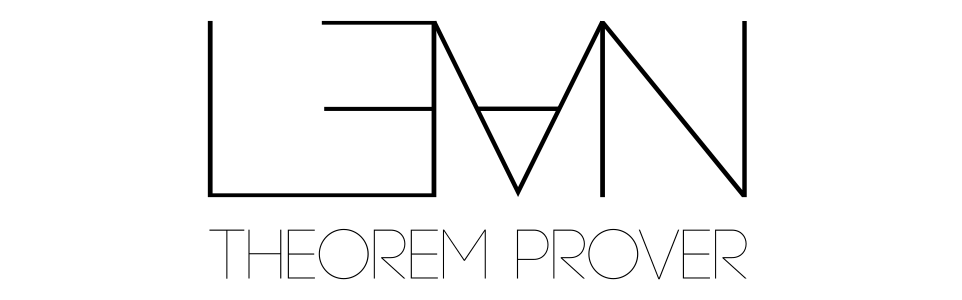
\includegraphics[height=0.8\titleimageht]{logo}
    }
}

\newcommand{\kit}[1]{\textcolor{KITgreen}{#1}}

\begin{document}

\begin{frame}{Towards a fully extensible frontend}
  Goal: \emph{democratize} frontend by removing the barrier between built-in and user-defined notions
  \vfill\pause
  \begin{itemize}
  \item extensible syntax from simple mixfix notations to character-level parsing
    \vfill\pause
  \item extensible semantics from simple syntax sugars to type-aware elaboration
    \begin{itemize}
    \item All levels covered by Racket-like macro hygiene (ITP'20)
    \end{itemize}
    \vfill\pause
  \item extensible tooling with access to frontend metadata
    \vfill
  \end{itemize}
\end{frame}

%\begin{frame}[fragile]{Frontend: overview}
%  \begin{center}
%    \begin{tikzpicture}[>=stealth, thick, nodes={rounded corners, minimum height=2em}, level distance=20mm]
%      \node[draw] {editor}
%      child[->] {
%        node[draw] (parser) {parser}
%        child {
%          node[draw]  (elab) {elaborator}
%          child[->] {
%            node[draw] {kernel}
%            edge from parent node[right] {core term}
%          }
%          edge from parent node[right] {concrete syntax tree}
%        }
%        edge from parent node[right] {string}
%      };
%      \draw[->,loop right] (elab) to node {concrete syntax tree} (elab);
%    \end{tikzpicture}
%  \end{center} 
%\end{frame}

\begin{frame}
  \vfill
  \begin{center}
    \Huge\textbf{Demo}
  \end{center}
  \vfill
\end{frame}

\end{document}

%%% Local Variables:
%%% mode: latex
%%% TeX-master: t
%%% TeX-engine: xetex
%%% TeX-command-extra-options: "-shell-escape"
%%% End:
